\documentclass[a4paper,8pt,twoside]{report}
\usepackage[portuguese]{babel}
\usepackage[utf8]{inputenc}
\usepackage{graphics}
\usepackage {color}
\usepackage{graphicx}
\usepackage{geometry}
\usepackage{flushend}
\usepackage[normalem]{ulem}              % para sublinhar texto
\usepackage{fancyhdr}                    % Para cabeçalhos
\usepackage{url}                         % Para tratar endereços 'url'
\usepackage{kpfonts}
\usepackage{latexsym}
\usepackage{hyperref}                 % For creating hyperlinks in cross references
\usepackage{amssymb}    
\usepackage {titlepic}       % carrega letras matemáticas


\begin{document}
\title{A Série e TV Guerra dos Tronos}

\author{Omeir Haroon}
\date {\today}

\begin{figure}[b]
\center
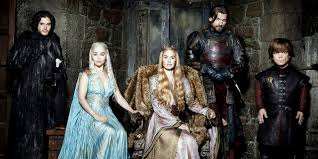
\includegraphics{got.jpeg}
\end{figure}


\maketitle
\chapter{Introducao}
\section{Sobre a série}\label{sec:intro}
A {\huge Guerra Dos Tronos}\footnote{Este nome é uma marca registada} é uma super producao televisiva da HBO, baseada na saga literária de George R.R. Martin, é uma série que { \footnotesize redefine os parâmetros do que é possível fazer em televisão}.

\vspace{1cm}


\begin{center}
\textit{ Uma narrativa épica que {\LARGE atravessa mundos imaginários} e personagens a perder de vista}\footnote{texto retirado de ... }
\end{center}

\vspace{1cm}

UPS! Este texto não devia estar aqui / § " % $ & ^  ~

\section{Elenco}\label{sec:lol}
A secção \ref{sec:intro} falou-nos sobre a série e agora na secção \ref{sec:lol} vamos falar sobre o elenco. tabela \ref{sec:intro} mostra-nos as personagens principais.

\begin{table}
	\centering	
	\begin{tabular}{|l|c|r|}
		\hline
		\textbf{Ator/Atriz} & \textbf{Personagem} & \textbf{Temporada}\\
		\hline
		Peter & Tryion & 1,2,3 \\
		\hline
		Emilia & Daenarys & 1,2,3 \\
		\hline
		Richard & Rob & 1,2,3 \\
	\end{tabular}
	\caption{Principais Personagens ao longo das temporadas}
\end{table}



\end{document}